\chapter{Experiment Result and Discussion}

\epigraph{Human memory is short and terribly fickle.}{\textit{Janine di Giovanni}}


This chapter provides the result and the analysis of the experiment. Three hypothesis are analyzed;
\begin{itemize}
  \item{Do participant experience the failure of prospective memory while using the smartphone?}
  \item{Is failure of prospective memory is more likely to happen with two intentions rather than one; intentional load matters}
  \item{Do increasing number of notification influence prospective memory error?}
  \item{Does mentally moving through event boundary increase the likeliness to experience failure of prospective memory?}
\end{itemize}

\section{Prospective memory error on smartphone}

\subsection{Experiment result}
In this experiment, the data from the participants from the three studies were combined.
Table \ref{fig:affirmationTable} shows who many participants believe that they had experienced prospective memory error,
and how many participants actually experience the prospective memory error during the experiment.
The participant was asked if they believe that they experienced prospective memory error using the first question on Table \ref{tab:demographicQuestion}.
The actual experience of memory error was calculated by looking if the people forget the questions during the experiment.

%The prospective memory error on the experiment is presented by the lost of intention during the study.
% The first column shows the affirmation on the prospective memory. the number is obtained by asking the participants \textit{"Often people go into a room to do something.  Though they know they intended to do something, they lose track of what they wanted to do.
% This same sort of thing can happen when using a smart phone, as well.  During the study,
% you may have clicked on a link, gone to the website, and then forgot what you intended to look up.  Did that happen to you at all during this study?"} on the post question phase during the experiment.
% While the second column is obtained by counting how many participant forget the question and chosed to look at the question again (lookback) during an experiment.
% The last column shows the total number of the participant participated on each study.
 %or forget the question during the experiment.

\subsection{Discussion}
% As seen in figure \ref{fig:demo1Study1}, \ref{fig:realdemo1Study1}, \ref{fig:demo1Study2}, \ref{fig:realdemo1Study2}, \ref{fig:demo1Study3}, \ref{fig:realdemo1Study3}, the left
% pie chart shows percentage of participant who think they are experiencing prospective memory error, and on the right side shows the percentage of participant who experience
% the prospective memory failure during the experiment.

Most of the participant did not believe that they have experienced the prospective memory error. In contrast, the output shows that  almost 70\% of the participant actually experienced the prospective memory error.
We can argue that the participant made an intention for looking the answer before clicking the answer link, but after reading the answer page
they lost their original intention.
As a result, they forget the content of the question, and they experience prospective memory error.
The result shows that while using a smartphone a person has a high probability of experiencing prospective memory error.
This experiment supports the result of Carlson's experiment.

% \begin{table}[]
% \centering
% \label{my-label}
% \begin{tabu}{|X[3,c]|X[3,c]|X[3,c]|}
% \hline
% \multicolumn{3}{|c|}{Study 1}                                                                             \\ \hline
% Affirmation of prospective memory error & \begin{tabular}[c]{@{}l@{}}Forget the questions \end{tabular} & Total Person \\ \hline
% 0                      & 3                                                                 & 4            \\ \hline
% \multicolumn{3}{|c|}{Study 2}                                                                             \\ \hline
% Affirmation of prospective memory error & Forget the questions  & Total Person \\ \hline
% 5                      & 8                                                                 & 11           \\ \hline
% \multicolumn{3}{|c|}{Study 3}                                                                             \\ \hline
% Affirmation of prospective memory error & Forget the questions                                            & Total Person \\ \hline
% 2                      & 2                                                                 & 3            \\ \hline
% \end{tabu}
% \caption{Participant affirmation and their experiment result on prospective memory error on smartphone}
% \label{fig:affirmationTable}
% \end{table}


\begin{table}[]
\centering
\small
\footnotesize
\begin{tabu}{|X[6,l]|X[2,c]|X[2,c]|X[2,c]|}
\hline
                                                                           & Experiment 1 (n=4) & Experiment 2 (n=11) & Experiment 3 (n=3) \\ \hline
How many participant believed they have experience prospective memory error & 0                  & 5                   & 2                  \\ \hline
How many participant actually experienced prospective memory error          & 3                  & 8                   & 2                  \\ \hline
\end{tabu}
\caption{Number of participant from all the studies who believed they have experince prospective memory error and the actual result of the experiment}
\label{fig:affirmationTable}
\end{table}



\section{The effect of multiple intention}

\subsection{Experiment result}
This section shows the result from the second study. On the second study, one or two questions were presented to the participant randomly.
Table \ref{fig:oneTwoQuestionForget} shows the total number of times the participant forgot the question and decided to see it again (lookback).
Each row shows how many times they did a loopback, percentage of loopback (p) and the total of the question.
The number of presented question was random, so the number of times the participant presented with
one or two question are not similar. Thus the percentage (p) is calculated by dividing the number of loopback with the frequency of one or two question
presented (N).
The table shows nine people forgot the question, six of them forgot more frequently if two questions are presented.
The last row shows that they forgot 31\% of the time if presented with two questions.
While they forgot only 8\% of the time if they presented with only one question.

Figure \ref{fig:TTFA_oneTwoQues} shows how long in millisecond each participant spent to write the answer (TTLFA).
The horizontal axis is the 11 participants and the vertical axis shows the duration of writing.
 It shows that 63\% (7 out of 11) spent longer time writing the answer if two questions were presented each time.

Figure \ref{fig:TTLFA_oneTwoQuesGeneral} shows the general mean of the writing time between one or two questions from all the participant.
It shows that if two questions were presented, then it will take longer time for the participant to write the answer.

Figure \ref{fig:lookingAnswer_oneOrTwo} shows the mean each participant spent on finding the answer on the answer page.
 The top plot was calculated on the first time they see the answer page.
 While the lower plot was calculated the second time they see the answer page after they decided to see the question again (loopback).
Surprisingly the top plot shows that almost half of the participants (4 out of 11) spent significantly longer time for one questions.
However. The lower plot shows that most of the participant spent longer time for two question.

\subsection{Discussion}

In this experiment, the intention of the participant was to find the answer and to write it
thus the number of questions presented is the number of intention need to be retained by the participant.
If the participant forget the question, we can argue that they experience loss of intention, as a result, they experience
prospective memory error \citep{Reason1984}.

Using this result we are trying to see  if an increasing the number of intention will make people more likely to experience failure of prospective memory
(is the intentional loads matter ?).
Based on the table \ref{fig:oneTwoQuestionForget}, a person more probable to experience prospective memory error if the amount of the intention was higher.
The result of this study shows that the amount of intentional loads are important component of prospective memory.

Furthermore, the result in figure \ref{fig:TTFA_oneTwoQues} and figure \ref{fig:TTLFA_oneTwoQuesGeneral} shows that the increasing amount intentional loads also
made the person harder to recall the content of the intention. the recall time is presented as the time participant write the answer.
On this analysis, the intention was to answer the question and it was formed after the participant found the answer.

In addition, based on figure \ref{fig:lookingAnswer_oneOrTwo}, the increasing amount of intention also increase the time
the participant spent on looking for the answer. This result shows that the number of intention decrease their cognitive performance.
This was probably because the increase of intentions reduced the level of attention while doing the task, and made
the participant spent longer time to find the answer.

\begin{table}[]
\centering
\small
\footnotesize
\begin{tabu}{|X[l]|X[l]|X[l]|}
\hline
\multicolumn{1}{|c|}{\multirow{2}{*}{Participant}} & \multicolumn{2}{c|}{Look the question again (Lookback)}                                         \\ \cline{2-3}
\multicolumn{1}{|c|}{}                             & \multicolumn{1}{c|}{one question} & \multicolumn{1}{c|}{two question} \\ \hline
1                                                  & 0 (p=0\%, N=2)                    & 0 (p=0\%, N=8)                    \\ \hline
2                                                  & 1(p=16\%, N=6)                    & 4 (p=100\%, N=4)                  \\ \hline
3                                                  & 0 (p=0\%, N=4)                    & 2 (p=33\%, N=6)                   \\ \hline
4                                                  & 1 (p=25\%, N=4)                   & 0 (p=0\%, N=6)                    \\ \hline
5                                                  & 0 (p=0\%,N=0)                     & 0 (p=0\%, N=10)                   \\ \hline
6                                                  & 0 (p=0\%, N=6)                    & 4 (p=100\%, N=4)                  \\ \hline
7                                                  & 0 (p=0\%, N=4)                    & 2 (p=33\%, N=6)                   \\ \hline
8                                                  & 1 (p=25\%, N=4)                   & 4 (p=66\%, N=6)                   \\ \hline
9                                                  & 0 (p=0\%, N=4)                    & 4 (p=66\%, N=6)                   \\ \hline
10                                                 & 1 (p=10\%, N=10)                  & 0 (p=0\%, N=0)                    \\ \hline
11                                                 & 0 (p=0\%, N=2)                    & 0 (p=0\%, N=8)                    \\ \hline
Total                                              & 4 (p=8\%,n=46)                    & 20 (p=31\%, n=64)                 \\ \hline
\end{tabu}
\caption{The number of lookback and its percentage (p) between one or two question from study 2}
\label{fig:oneTwoQuestionForget}
\end{table}

% Hampir 75\% dari kelupaan adalah two questions.
%
% then show that TTLFA time they write the answer also longer
% then show that using two question make people look at the answer longer time,
% turns out not. but most of the time participant look again the answer for two question

\begin{figure}[!h]
\centering
\begin{minipage}{.5\textwidth}
  \centering
  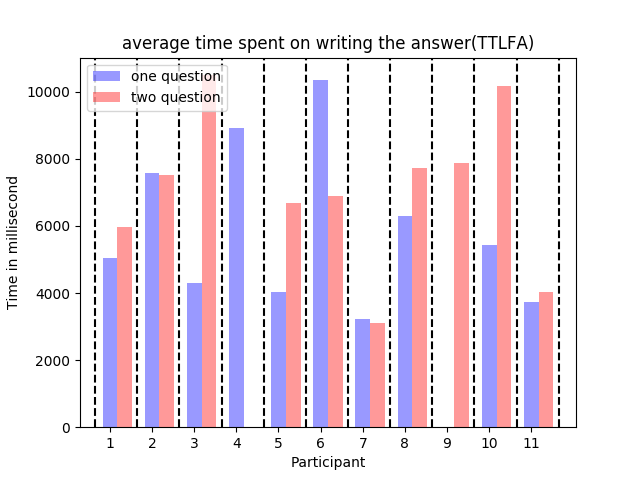
\includegraphics[scale=0.5]{TTFLA_each_participant}
  \captionsetup{justification=centering}
  \captionof{figure}{Mean time filling the answer of each participant between one or two question in study 2}
  \label{fig:TTFA_oneTwoQues}
\end{minipage} \qquad
\begin{minipage}{.5\textwidth}
  \centering
  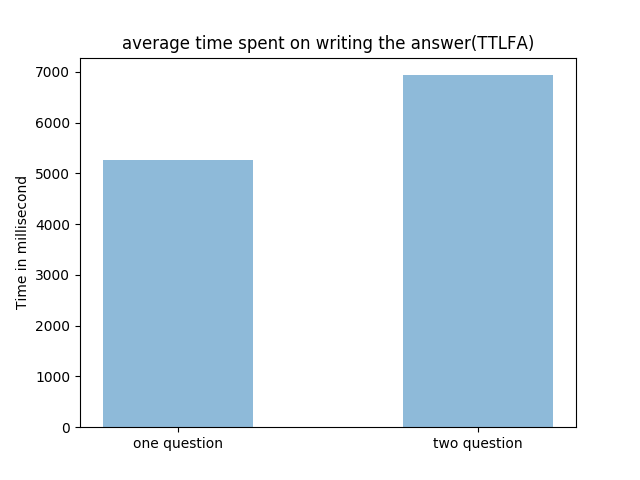
\includegraphics[scale=0.5]{TTLFA_general}
  \captionsetup{justification=centering}
  \captionof{figure}{Mean time filling the answer of all the participants between one or two question in study 2}
  \label{fig:TTLFA_oneTwoQuesGeneral}
\end{minipage}
\end{figure}


\begin{figure}[!h]
\begin{center}
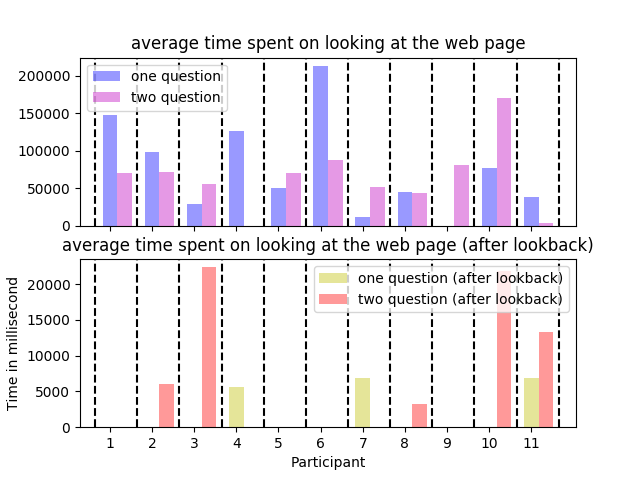
\includegraphics[scale=0.86]{visitedLink_each_participant}
\end{center}
\captionsetup{justification=centering}
\caption{Mean time in spent finding for an answer between one or two questions}
\label{fig:lookingAnswer_oneOrTwo}
\end{figure}


% \begin{table}[]
% \centering
% \caption{My caption}
% \label{my-label}
% \begin{tabular}{|l|l|l|l|l|l|l|l}
% \cline{1-7}
% \multirow{2}{*}{Question}           & \multicolumn{2}{l|}{Study 1} & \multicolumn{2}{l|}{Study 2} & \multicolumn{2}{l|}{Study 3} &  \\ \cline{2-7}
%                                     & Yes           & No           & Yes           & No           & Yes           & No           &  \\ \cline{1-7}
% Experience prospective memory error & 0             & 4            & 5             & 6            & 2             & 1            &  \\ \cline{1-7}
% Forget about the answer             & 2             & 2            & 4             & 7            & 0             & 3            &  \\ \cline{1-7}
% \end{tabular}
% \end{table}

% Please add the following required packages to your document preamble:
% \usepackage{multirow}


\section{The effect of notification}
\subsection{Experiment Result}
Table \ref{tab:notifiactionNumber} shows the mean time participant spent on writing the answer (TTLFA), mean time finding the answer
and the percentage of looking the question again (lookback). The variables are grouped by the number of notification received.
It shows that increase in the number of notification make people spent more time writing and finding the answer.
However, the number of notification does not have correlation with the percentage of lookback.

\begin{table}[]
\centering
\small
\footnotesize
\begin{tabu}{|X[l]|X[l]|X[l]|X[l]|}
\hline
                  & Mean time to write the answer (TTLFA) & Mean time spent on looking for an answer & Forget the question (lookback) percentage \\ \hline
No Notifications  & 6.267 second                     & 59.875 second                       & 17\%               \\ \hline
One Notification  & 7.292 second                     & 69.517 second                       & 11\%               \\ \hline
Two Notifications & 7.304 second                     & 76.699 second                       & 21\%               \\ \hline
\end{tabu}
\caption{The result of different number of notification received by the participant from all studies}
\label{tab:notifiactionNumber}
\end{table}


\subsection{Disscussion}
This result shows that the notification does not have any effect on the prospective memory error.
Table \ref{tab:notifiactionNumber} shows that the increasing number of notification made the participant spent longer time
to write and to find an answer. Because in this experiment the notification appeared when the participant looks
at the question and find the answer. Then the

If the notification appeared when the person is looking for the answer then the result
is consistent with the time needed to pay attention and to dismiss the notification.
Thus we can not draw a conclusion based on the time spent looking for the answer.

However, the notification did not appear when a participant was writing the answer hence we can analyze this variable.
In this analysis, we argue that the intention is writing the answer and the content
is the answer itself. Therefore the notification makes them harder to recall the content of the intention.
Probably because the notification act as a distraction that lower the level of attention when the intention is framed to the memory.

%
% If the notification is shown when the participant presented with the question,
%  then the notification probably lower the level of attention thus make the intention not framed perfectly.
% But if the notification is shown when the participant find the answer, this can mean that the notification attenuate the content of intention,
% even though it's correctly framed before.

% In addition, if we consider the notification as an event boundary. We can argue that
% that mentally moving through event boundary will influence the intention but has no effect on the prospective memory error.

\subsection{Event boundary on prospective memory}
\subsection{Experiment Result}
The bar chart \ref{fig:lookingAnswer_lookback} shows the mean time (in millisecond) the participants spent finding the answer on the answer page.
The chart shows the participant who forgets the question (lookback) had spent more time finding the answer before decides to see the question again.
The bar chart \ref{fig:freq_study1} and \ref{fig:freq_study3} shows how many time the participant saw question again (lookback) on each question, it shows the data from first and the third study respectively.
the bar charts show that the more participants forget the question on the third study.
Table \ref{visitedPage} shows the number of web page participant visit by click link inside the web page, and the number of times participant forget the question (lookback).
for the visited link that has zero value, this is probably because the participant did not click the answer links or the application fails to track the data.
% The bar chart \ref{fig:aveTime_study1} and \ref{fig:aveTime_study3} shows the time spent looking for the answer on each questions, it shows the data from first and the third study respectively.
% It shows that the participant spent longer time to look at the answer and they spent longer time to look at the answer again after the do lookback.
\begin{figure}[!h]
\begin{center}
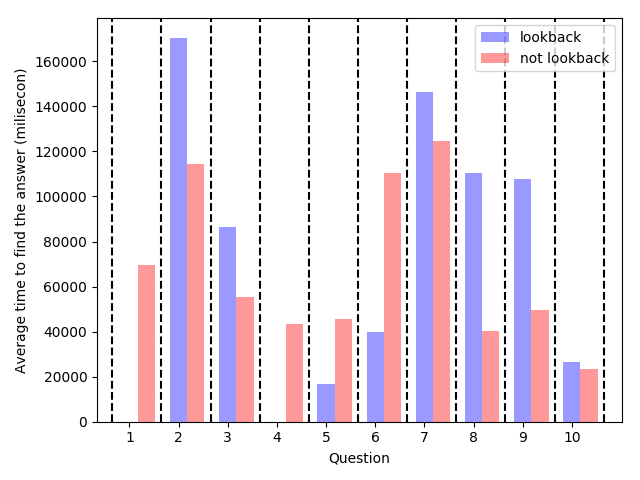
\includegraphics[scale=0.86]{lookback_and_reading_time_studyAll}
\end{center}
\captionsetup{justification=centering}
\caption{Mean time in spent looking for an answer between lookback and non-lookback in all studies}
\label{fig:lookingAnswer_lookback}
\end{figure}

\begin{figure}[!h]
\centering
\begin{minipage}{.5\textwidth}
  \centering
  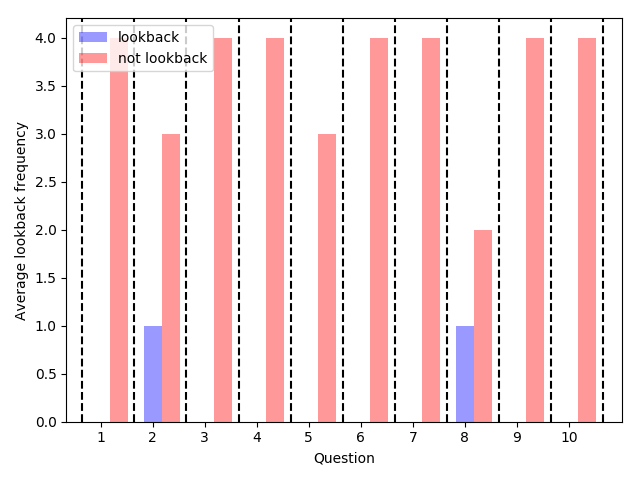
\includegraphics[width=\textwidth]{frequency_lookback_study1}
  \captionsetup{justification=centering}
  \captionof{figure}{Frequency of lookback of the participant on study 1}
  \label{fig:freq_study1}
\end{minipage}%
\begin{minipage}{.5\textwidth}
  \centering
  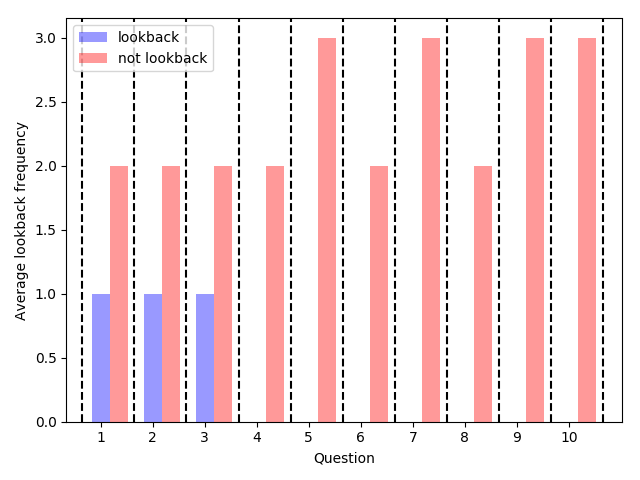
\includegraphics[width=\textwidth]{frequency_lookback_study3}
  \captionsetup{justification=centering}
  \captionof{figure}{Frequency of lookback of the participant on study 3}
  \label{fig:freq_study3}
\end{minipage}
\end{figure}

% \begin{figure}[!h]
% \centering
% \begin{minipage}{.5\textwidth}
%   \centering
%   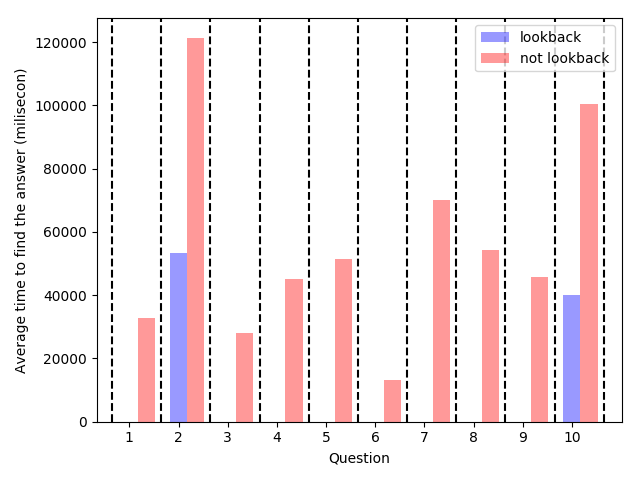
\includegraphics[width=\textwidth]{lookback_and_reading_time_study1}
%   \captionsetup{justification=centering}
%   \captionof{figure}{Mean time of all the participants spent finding the answer in study 1}
%   \label{fig:aveTime_study1}
% \end{minipage}%
% \begin{minipage}{.5\textwidth}
%   \centering
%   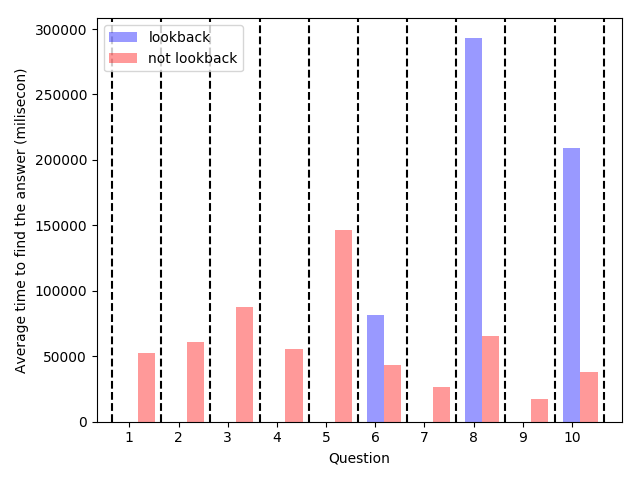
\includegraphics[width=\textwidth]{lookback_and_reading_time_study3}
%   \captionsetup{justification=centering}
%   \captionof{figure}{Mean time of all the participants spent finding the answer in study 3}
%   \label{fig:aveTime_study3}
% \end{minipage}
% \end{figure}


\begin{table}[!b]
\centering
\small
\footnotesize
\begin{tabu}{|X[3,l]|X[5,l]|X[5,l]|X[3,l]|}
\hline
Number of visited links & number of times participant forget the question (lookback)(N=192) & number of times participant,remember question(N=192) & SUM \\ \hline
0                       & 9                                                                 & 6                                            & 15             \\ \hline
1                       & 35                                                                & 135                                          & 170             \\ \hline
2                       & 1                                                                 & 5                                            & 6           \\ \hline
3                       & 0                                                                 & 1                                            & 1        \\ \hline
SUM                   & 45                                                                  & 147                                          & 192 \\ \hline
\end{tabu}
\caption{Number of visited page and how many times participant forget or remember the question from all the studies}
\label{visitedPage}
\end{table}


\subsection{Discussion}
A participant experienced a transition through event boundary after they move from one view to another view on the smartphone.
In this discussion the transition happened two times; when the participant saw the question then clicked the button then the application changed to answer link view,
and when the person clicked the answer link then the application changed to the answer page view.
During this transition, the participant still retained the intention which was looking for the answer.

The result of the bar chart \ref{fig:lookingAnswer_lookback}  shows that the participants who experienced prospective memory error had spent more time finding the answer.
We can argue that when they were reading the answer page, they forgot the intention (lost intention) or forgot the content of the intention (detached intention) which result in prospective memory error.
This happened probably because the amount of new information they received during reading reduce the retention level of the intention \citep{Reason1984}.
We can also argue that a new information mentally create a new event boundary. So the longer time they spent reading the web page, more mental transition happened.
This moving through more event boundary makes a person more likely experience prospective memory error.

However, if we consider moving through a new web page as a transition between event boundary. Table \ref{visitedPage} shows that there was no correlation between a mental transition to prospective memory error.
But this view is very weak since most of the participant only visited one web page.

To understand the effect of physical transition through event boundary, we try to investigate the frequency of prospective memory error between first in the third study.
Bar chart \ref{fig:freq_study1} and \ref{fig:freq_study3} shows that the participant on the third study forgot the question more frequently than the first study. However,
we can only see the probability that physical transition will increase the likeliness of prospective memory failure, but
we cannot draw a strong correlation because the sample is very small.
This possibility contradicts the result from Carlson experiment.
Over all, the results on this discussion section support the event horizon model proposed by \cite{Radvansky2006}.
% However, by looking at bar charts \ref{fig:aveTime_study1} and \ref{fig:aveTime_study3} we can see that the physical transtition r
% esult on the longer time for people to read and find the answer.
% This shows that the physical transition decrease the capability of cognitive ability while doing this experiment.
